\documentclass[a4paper,11pt]{article}
\usepackage[english]{babel}
\newcommand{\sectionbreak}{\clearpage}
\usepackage{titlesec}
\usepackage{listings,xcolor}
\lstset{
language=Python,
keywordstyle=\color{blue},
commentstyle=\color{green},
stringstyle=\color{red},
numberstyle=\tiny\color{gray},
}
\usepackage{graphicx}
\begin{document}
\title{Python Project Document}
\author{150101027- I.N.Dilip Kumar\\ 150101051- Hareesh Reddi\\ 150101032- L.Sai Shobith}
\date{\today}
\maketitle
\tableofcontents{}
\section{Introduction}
In the given attack data file, each category has 10 directories. We select 7 directories for the training and use the other 3 directories for testing. \newline
The problem statement is:

Split the Attack data of each category (Hydra-FTP, Hydra-SSH, Adduser, Java-Meterpreter, Meterpreter and Webshell ) into 70\% training data and 30 \% test data. For instance there are
are 10 folders in "Adduser" attack. Therefore, 7 of these folders are to be used for training and 3 folders are to be used for testing.

For the Normal data, files in "Training\_Data\_Master" folder are to be used as training data and files in "Validation\_Data\_Master" folder are to be used as test data.

Write a python script to find the frequency of occurences of all unique 3-grams, 5-grams and 7-grams system call sequences in the training data for both Attack data (across all categories of attack) and Normal data.

Perform the same task on files in the \"Training\_Data\_Master\" to obtain all the unique 3-grams, 5-grams and 7-grams.

Once you have obtained the frequencies of all the unique n-grams terms in the training data,use the top 30\% n-grams terms with the highest frequency to create a data set.

Apply the same procedure to generate the test dataset from the test files of the attack data (for all attack types) and the normal files in the "Validation\_Data\_Master" using the top 
30\% 3-grams terms with highest frequencies obtained during the training phase. The classifier model developed during the training phase will finally be validated on the Test dataset.

\section{Algorithm}
\begin{enumerate}
\item Select the first seven folders for each category and find all the text files in all the directories.
\item Find all the seven grams for each file.
\item Find the frequency of each seven gram and keep them in a dictionary.
\item Using the seven grams, find the 5 grams and 3 grams by taking the first three numbers for 3 gram and first five for 5 gram.
\item Find the frequency for each of the 5 grams and for 3 grams and keep them in a dictionary.
\item Sort the dictionary based on the values as frequencies.
\item Select the top 30 percent of the n-grams and do this for each category and for the training data set.
\item Concat all of the top 30 percent n-grams and keep them in a single dictionary and let us call it feature file.
\item Now for each text file in the test data and validation data master create another text file which contains the 7 gram in the feature file and if it is in the text file write it's frequency and if it is not present write 0 as the frequency.
\end{enumerate}

\section{Algorithm Analysis} 
\begin{enumerate}
  \item  O(No.Of.TextFiles) is the time complexity of first step 
  \item  O(No.Of.SevenGrams) is the time complexity of second step
  \item  O(No.Of.SevenGrams) is the time complexity for finding the frequencies and O(NlogN) where N is No.Of.SevenGrams for sorting the dictionaries
  \item  O(No.Of.ThreeGrams + No.Of.FiveGrams)\textless=O(No.Of.SevenGrams) for the fourth step
  \item  O(No.Of.ThreeGrams + No.Of.FiveGrams) is the time complexity of fifth step
  \item  O(NlogN) where N is No.Of.SevenGrams is time complexity for sorting the dictionaries 
  \item  O(N) where N is No.Of.SevenGrams is time complexity for selecting the top 30\% N-Grams from the dictionaries
  \item  O(N) where N is No.Of.SevenGrams is time complexity for concatenating the dictionaries
  \item  O(N*No.Of.TextFiles) is the time complexity for the ninth step
\end{enumerate}

\section{Code Description}
This is the code description

\subsection{Section1}
The unify(“Adduser”) will return three dictionaries of 7 tuples, 5tuples, 3tuples as keys and their frequencies as values
\begin{figure}[ht!]
\centering
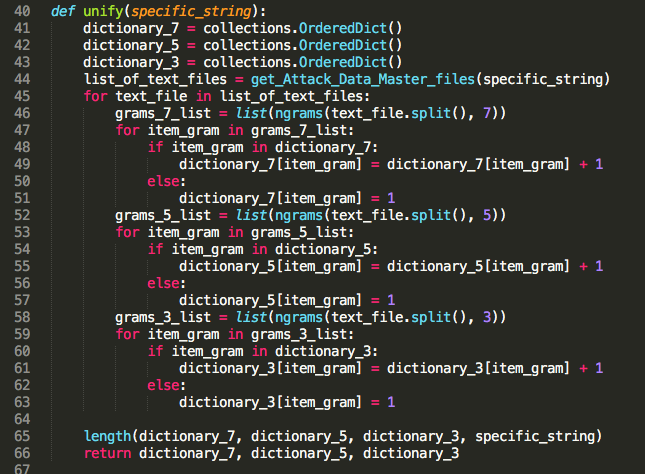
\includegraphics[width=90mm]{4.png}
\caption{Fig1\label{ooo0o}}
\end{figure}

\subsection{Section2}
The Sorted() function will sort the dictionary based on their values in decreasing order and returns the list of keys in that order
\begin{figure}[ht!]
\centering
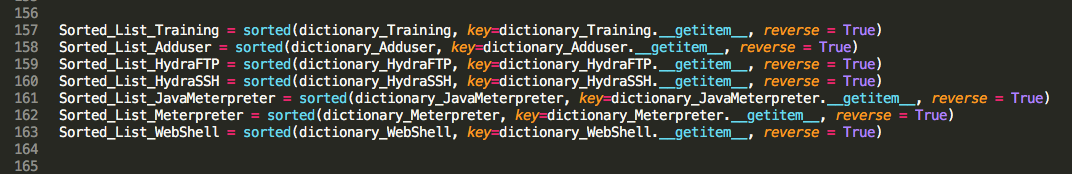
\includegraphics[width=90mm]{3.png}
\caption{Fig2\label{oooo}}
\end{figure}

\subsection{Section3} \newpage
The Sorted\_List\_Adduser is a list which contains the tuples in sorted order of their frequencies
The same process above is done for each type of attack
\begin{figure}[ht!]
\centering
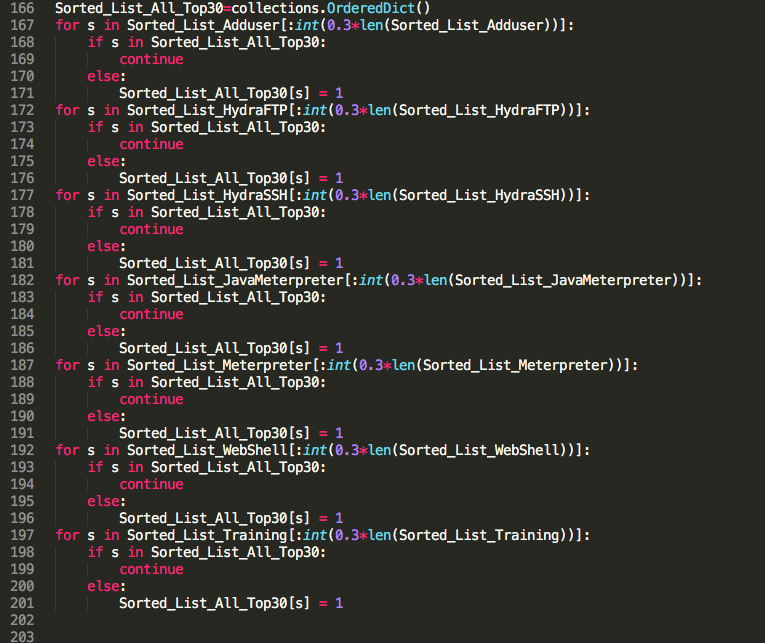
\includegraphics[width=90mm]{2.png}
\caption{Fig3\label{ooo}}
\end{figure}

\subsection{Section4} \newpage
A dictionary is formed with tuples whose frequencies are top 30 percent in the sorted dictionary for each kind of attack and concatenated into one and is called the feature set
Now the feature set is tested against each file in the Adduser folder and a file is created in which if the tuple in the feature set is present in the n-grams of the selected file then the n-gram and it’s frequency in the selected file is printed, if it is not present then it will print the n-gram and 0 as the frequency
The same is done for 5 gram and 3 gram

\begin{figure}[ht!]
\centering
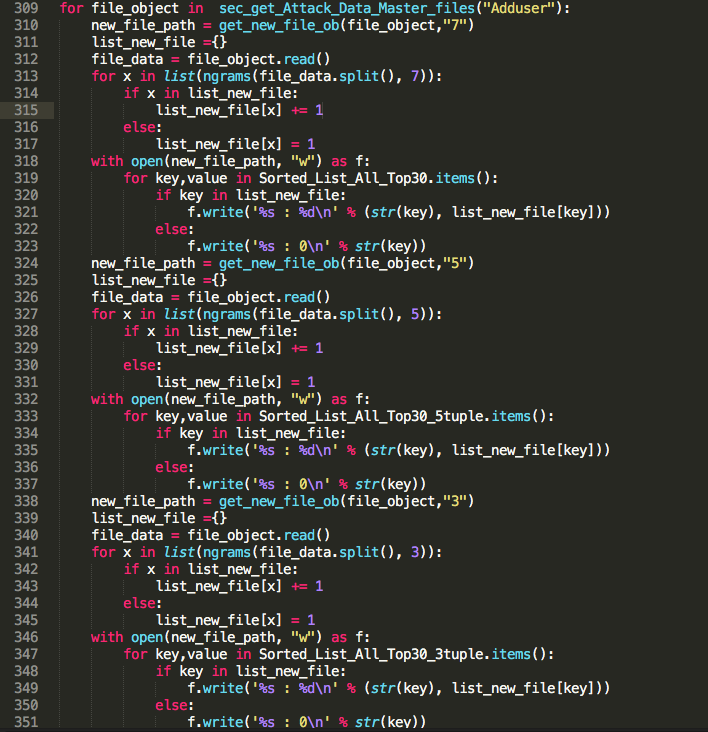
\includegraphics[width=90mm]{1.png}
\caption{Fig4\label{ooo}}
\end{figure}

\end{document}